\documentclass{article}
\usepackage{amsmath, amssymb, amsthm, enumerate, url}
\usepackage{graphicx}

\title{Using Closed-Loop Detection to Improve Homography Estimation and Mosaicing}
\author{Michele Pratusevich}
\date{\today}

\begin{document} 
\maketitle
\tableofcontents

%\begin{abstract}
%
%The goal of the project is to improve automatic image mosaicing. An image
%mosaic is constructed by splitting a video of a scene into images and computing
%image homographies between adjacent videos. However, errors in the homography
%computation compound with each homography computation, resulting in inaccurate
%mosaicing. The image sequence is analyzed to detect closed loops, or when the
%image returns to a component in the scene that has already been seen. Using the
%information from a detected closed loop, the homographies computed from the
%images are improved for accuracy.      
%
%\end{abstract}

\section{Introduction and Overview}

The goal of this project is to improve an automatically mosaiced image by
detecting a closed loop in a sequence of images and re-computing the calculated
image homographies using nonlinear optimization. First homographies will be
discussed, with some discussion about factoring homography matrices to
determine the various components of a homography. Next the techniques for
detecting a closed loop in an image sequence are discussed. Then the
optimization problem for improving the homography matrices is described in
terms of formulation and the constraints. Lastly, further considerations and
ideas are discussed. 

The high-level structure for the process of correcting an image mosaic using
closed loop information is as follows:

\begin{figure}[h!]
\centering
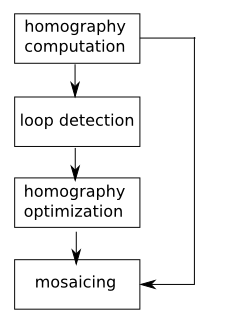
\includegraphics[width=3cm]{highleveldiaf.png}
\caption{The high-level work flow for optimizing the image mosaic.}
\end{figure}

\section{Homographies}

\subsection{In General} 

A homography $H$ in this context is a $3$ by $3$ matrix $H_{i, j}$ that
describes the relationship between image $i$ and image $j$ in an image
sequence. In this application, the homographies $H_{i, i + 1}$ are calculated
between consecutive images $i$ and $i + 1$. When calculating an image mosaic,
the cumulative homography for image $k$ in the sequence is calculated by
multiplying each of the previous homography matrices together until the current
image: 

\[H_{1, k} = H_{1, 2} \cdot H_{2, 3} \cdots H_{k - 1, k}\]

In the application of creating a 2-D mosaic from a video, the homography is a
2D homography, transforming a point $[u, v, 1]^T$ to $[u', v', 1]^T$ up to a
scale factor, normalized in OpenCV to be $1$. 

\subsection{Factoring a Homography Matrix}
\label{factoring}

As discussed by Sonka, et. al in \cite{sonkatext}, homographies form a group
under multiplication as shown above. There are various important subgroups that
can be used to factor any homography matrix $H$ into it's components. As
discussed in \cite{sonkatext}, any homography can be decomposed as $H = H_P H_A H_S$ where 

\[
H_P = \begin{bmatrix} I & \mathbf{0} \\ \mathbf{a}^T & b \end{bmatrix}, \qquad
H_A = \begin{bmatrix} K & \mathbf{0} \\ \mathbf{0}^T & 1 \end{bmatrix}, \qquad
H_S = \begin{bmatrix} R & -R\mathbf{t} \\ \mathbf{0}^T & 1 \end{bmatrix}
\] 

And $K$ is upper triangular. Page $557$ in \cite{sonkatext} gives more
information about these subgroups. 

Using the factorization above as a starting point, a homography matrix is
therefore written as follows:

\[H = H_P H_A H_S = \begin{bmatrix}KR & -KR\mathbf{t} \\ \mathbf{a}^TKR &
 -\mathbf{a}^TKR\mathbf{t} + \mathbf{b} \end{bmatrix}\] 

Where $t$ is the translation vector, $R$ is the rotation matrix for rotation in
the $xy$-plane, and $K$ is the dilation matrix in the $xy$-directions.
$\mathbf{a}$ and $\mathbf{b}$ are coefficients related to the rotation and
dilation in the $z$ direction.

\subsection{Computing the Homography Matrices in Code: Overview}

The homography matrices can be computed using an OpenCV method called
\verb|cvFindHomography|, described in \cite{cvhomogs}, which needs to be tuned
according to the application you are working with. For instance, the window
size that is needed to find a correct homography depends on how close the
camera is to the scene in question. 

To use the \verb|cvFindHomography| method you already need to have points
picked out on both images that are known to be correspondent. In applications
with few images, these points can be picked out by hand and visual inspection.
Because the goal of this project was to create a fully automated mosaicing
algorithm, manually picking points was not an option. Instead, because the
image sequence is taken from a video, the video can be sequenced in such a way
to make the images overlapped by a significant amount. Given this information,
we use optical flow in the OpenCV method \verb|cvCalcOpticalFlowPyrLK| to
calculate the new positions of interest points from the first image in the
second image, described in \cite{opticalflow}. The optical flow method has parameters to tune as well. 

The interest points in the first image are found using the OpenCV methods
\verb|cvGoodFeaturesToTrack| and \verb|cvFindCornerSubPix|, described in
\cite{points}. The parameters on these methods must be tuned as well. 

The \verb|cvFindHomography| method then uses correspondences in those points to
compute an image-wide homography that is then used to construct the mosaic. 

The code is given in \ref{apdx:code} and the information about adjusting
parameters in all the functions is given in \ref{apdx:params}.

\section{Mosaicing}

Mosaicing is the process of stitching images together to form a larger image.
The homographies that were calculated between consecutive images are applied to
each of the images in turn on a black canvas, overlapping the images in the
same frame. The method \texttt{drawMosaic3} from the DOLBA project code was
used for the image mosaicing step.  

\section{Detecting a Closed Loop}

\subsection{Overview}

The general idea is to detect the presence of a closed loop in an image
sequence using information from the images alone, that is not very
computationally intensive. To mosaic images, the homography between them must
be computed, so finding a way to use the already-computed homography matrices
to determine the presence of a closed loop is a good use of information that is
already computed. 

\subsection{Method}
\label{sec:subm}

Based on the factorization of a homography discussed in section \ref{factoring},
various components of a homography matrix can be factored out and used in an
algorithm to detect a closed loop. There are a number of approaches you can
take, all of which I will describe here.

\begin{enumerate}

\item \textbf{Submatrix of homography matrix}

According to the factorization described in section \ref{factoring}, the
subvector in the top right corner of the homography matrix (entries $(1, 3)$
and $(2, 3)$) represents $-KR\mathbf{t}$ and could be used as an approximation
to the translation. 

\item \textbf{Cumulative translation vector} 

The general idea is this: when you factor each homography matrix $H_{i, i + 1}$
as you compute it between two consecutive images, you compute the translation
change $\mathbf{t}_{i, i + 1}$. Keep track of a cumulative translation vector
$\mathbf{t}_{1, k}$ by adding each of the previously-computed translation
vectors. The translation vector computed is the ``general translation'' for
that particular homography. It does not necessarily represent the translation
of the center of the image - it represents the ``average'' (for some sense of
the word average) translation between the image and the previous image. If the
translation component of each pixel in the image were to be computed, the
translation vector would represent the average of all these vectors.

To compute the translation vector $\mathbf{t}$ use the following steps:

\begin{itemize}

\item First compute $-KR\mathbf{t}$ by taking the $(1, 3)$ and $(2, 3)$ entries
in the $H_{i, i + 1}$ matrix.

\item Next compute $KR$ by taking the $2$ by $2$ submatrix of $H_{i, i + 1}$
that starts in the top left corner.

\item Compute the inverse of $KR$.

\item Using this vector and matrix, $\mathbf{t} = -(KR)^{-1}(-KR\mathbf{t})$.  

\end{itemize}

To see the code excerpt for computing $\mathbf{t}$, refer to Appendix \ref{apdx:t}.

The translation for the first image is $(0, 0)$ (since the homography for the
first image is the identity matrix), so the other translation vectors can be
thought of as the new position of the center of the image. Really it is the new
position of the center of mass of the image, but thinking of it as the
translation of the center is a good approximation. 

\item \textbf{Translation vector from cumulative homography}

Instead of factoring the homography matrices between images $i$ and $i + 1$,
use the computed cumulative homography matrix in the same way (factoring) to
extract the translation estimation from the cumulative homography, instead of
needing to keep track of the cumulative translation. Much like in the previous
option, factor $\mathbf{t}$ from the submatrices of the cumulative homography
matrix.  

\end{enumerate}

\subsection{Closed loop metric}
\label{sec:clmetric}

Regardless of which method is used to compute the ``translation'', the method
and metric for determining whether there is a closed loop in the image is the
same. 

To determine whether there is a closed loop in the image, use the translation
vector approximation determined using one of the techniques described above. If
the new center of the image falls within the maximally-inscribed ellipse
inscribed in the first image, then it is possible that enough of the second
image overlaps with the first image to compute a new homography. That is, if

\[\mathbf{t} = \begin{pmatrix} t_x \\ t_y \end{pmatrix}\]

And if 

\[\frac{t_x^2}{(\frac{\textnormal{imgWidth}}{2})^2} + \frac{t_y^2}{(\frac{\textnormal{imgHeight}}{2})^2} \leq 1\]

Then image $i + 1$ overlaps with the first image in the sequence.

\subsubsection{Problems and a correction factor}

There are some problems with this approach of attempting to determine the
presence of a closed loop from the computed image homographies.

The problem that this approach is initially meant to solve makes the estimation
of the true translation vector difficult, mainly because the homography
computations inherently are error-prone. The summation of translation vectors
from image to image just compounds the error present in each of the individual
homography computations. 

This means that the estimation of the center of the image from the cumulative
translation vector is not completely accurate, so there needs to be some kind
of correction factor in the elliptical equation to account for the drift in the
homographies. So the actual equation used to determine whether there is an
overlap between the current image and the first image is

\[\frac{t_x^2}{(\frac{\textnormal{imgWidth} \cdot \textnormal{scaleFactor}}{2})^2} + \frac{t_y^2}{(\frac{\textnormal{imgHeight} \cdot \textnormal{scaleFactor}}{2})^2} \leq 1\]

Using a scale factor of $1.5$ yields good results, yielding many false
positives. However, having strict conditions to enter the optimization phase
alleviates the need to minimize false positives in closed loop detection. In
fact, the more potential closed loops that are detected, the more opportunity
for optimization and adjustment. So if an image is prematurely detected as
overlapping with the original image and ends up satisfying the criteria for
entering the optimization phase, then the mosaic will be adjusted earlier.

\subsection{Translation tracking examples}

The following are two examples of tracking the centers of the images using the
algorithms detected above. 

In this example, there are $49$ images in this closed loop sequence. 

\begin{figure}[ht!]
\centering
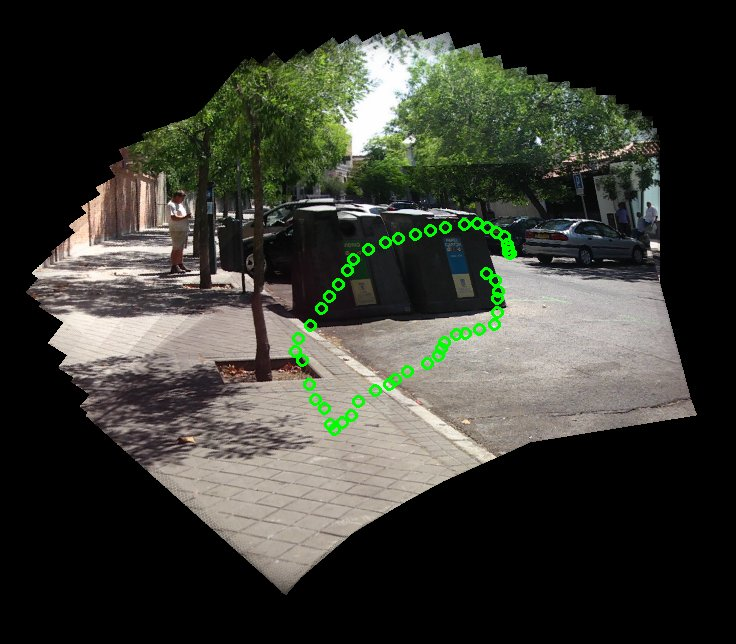
\includegraphics[width=6cm]{centers_imgs/test_set_15_nKRt_YES/moswithtrans0049_edit.jpg}
\caption{Computed using the submatrix of the cumulative homography matrix}
\end{figure} 

\begin{figure}[ht!]
\centering
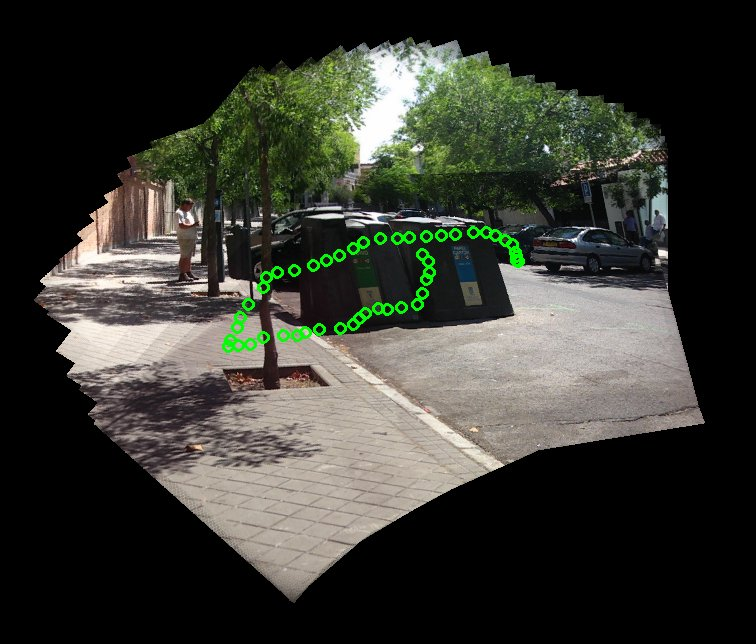
\includegraphics[width=6cm]{centers_imgs/test_set_15_tcum_YES/moswithtrans0049_edit.jpg}
\caption{Computed using the cumulative translation vector}
\end{figure}

\begin{figure}[ht!]
\centering
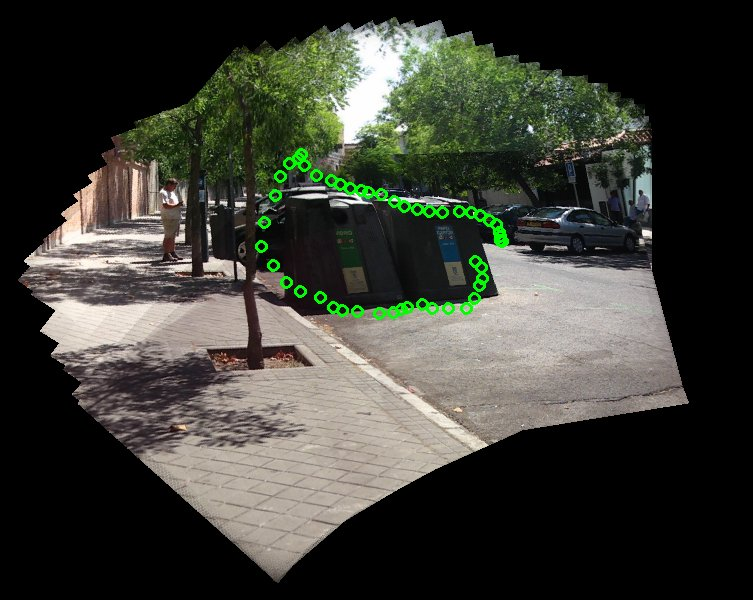
\includegraphics[width=6cm]{centers_imgs/test_set_15_t_from_h_all_YES/moswithtrans0049_edit.jpg}
\caption{Computed using the translation vector from the cumulative homography}
\end{figure}

From these three images it is evident that any of these three methods can be
possible valid ways of estimating the translation vector from the homography
matrices. Determining the most effective method for determining closed loops
would require more test data sets and running many tests, comparing against a
standard metric. 

\subsection{Another closed-loop estimation possibility}

A potential possibility for determining the presence of a closed-loop is to use
the same overlap metric as described in Section \ref{sec:clmetric} but using a
different technique altogether for estimating the translation component of the
images.

In this technique, instead of using homography decomposition and factoring, the
idea would be to use computation to estimate the positions of the centers of
the images using direct transformation. The center of the first image would be
without loss of generality assumed to be at $(0, 0, 1)$ (because all vectors
are in 3D space). When the cumulative homography for image $k$ ($H_{1, k}$) is
calculated, it will be multiplied to this center vector to determine the
position of the new center. However, this technique is actually the same as
using the submatrix from the cumulative homography matrix as described in
Section \ref{sec:subm}, because multiplying the homography matrix by $(0, 0,1)$ 
will just yield the $(1, 3)$ and $(2, 3)$ entries of the matrix. So there
is no need to try this method as a way of estimating image translation vectors.  

\section{Optimization Problem Formulation}

This is the problem formulation for the optimization problem in closed-loop
homographies.

There is a closed loop detected between image $1$ and image $n$. Each
homography computed by the mosaicing algorithm, $H_{i, i + 1}$, is the
homography from image $i$ to the next image $i + 1$, computed using OpenCV (and
RANSAC). Once the closed loop is detected, the homography $H_{1, n}$ is
computed between image $1$ and the overlap image $n$. 

There are two possible formulations of the optimization that I will discuss. I
have tried both of them to varied success, as I will also describe with each
section. 

\subsection{Objective Function Minimizing the Cumulative Error}

Overall, the goal of the optimization algorithm is to minimize the error
between
 
\[H_{1, 2} \cdot H_{2, 3} \cdots H_{n - 2, n - 1} \cdot H_{n - 1, n} - H_{1, n} = 0\]

Which can be written as

\[H_{1, n}^{\textnormal{cumulative}} - H_{1, n} = 0.\]

\subsubsection{Objective function}

Using a scalar formulation of the problem, the error is calculated by
calculating the sum of the squares of the differences between the
cumulative and new homographies for each component in the matrix.

\[\sum_{i,j} ((H_{1, n}^{\textnormal{cumulative}})_{ij} - (H_{1, n})_{ij})^2.\]

The variables given to the optimizer are the $8$ parameters in each of the
matrices $H_{i, i + 1}$ (each entry of the homography matrix except for the $3,
3$ entry, which is assumed to be $1$. The values of the $H_{1, n}$ matrix are
not variables in the optimization function, but are taken as truth.
\footnote{It is possible to use the components of the closed-loop matrix as
variables too, but for now I've implemented the code to consider it as truth. I
will try using those components as variables as well.} The optimizer will yield
$n$ new homography matrices $H_{i, i+1}^{\textnormal{optimized}}$. 

\subsubsection{Constraints}

The optimizer tries to minimize this nonlinear multivariable function according
to the following constraints:

\begin{enumerate}

\item The variables in each matrix can't change ``too much.'' There are a few
ways to implement this:

\begin{enumerate}

\item \label{indiv_thresh} The individual variables can only change within a certain range (with
this range being different depending on which component in the homography it
is):

\[((H_{i, i+1})_{1, 1} - (H_{i, i+1}^{\textnormal{optimized}})_{1, 1})^2 \leq \textnormal{change\_threshold}\] 
\[((H_{i, i+1})_{1, 2} - (H_{i, i+1}^{\textnormal{optimized}})_{1, 2})^2 \leq \textnormal{change\_threshold}\] 
\[((H_{i, i+1})_{2, 1} - (H_{i, i+1}^{\textnormal{optimized}})_{2, 1})^2 \leq \textnormal{change\_threshold}\] 
\[((H_{i, i+1})_{2, 2} - (H_{i, i+1}^{\textnormal{optimized}})_{2, 2})^2 \leq \textnormal{change\_threshold}\] 
\[((H_{i, i+1})_{3, 1} - (H_{i, i+1}^{\textnormal{optimized}})_{3, 1})^2 \leq \textnormal{pixel\_threshold}\] 
\[((H_{i, i+1})_{3, 2} - (H_{i, i+1}^{\textnormal{optimized}})_{3, 2})^2 \leq \textnormal{pixel\_threshold}\] 
\[((H_{i, i+1})_{1, 3} - (H_{i, i+1}^{\textnormal{optimized}})_{1, 3})^2 \leq \textnormal{small\_threshold}\] 
\[((H_{i, i+1})_{2, 3} - (H_{i, i+1}^{\textnormal{optimized}})_{2, 3})^2 \leq \textnormal{small\_threshold}\] 

The reason each entry (or group of entries) should have it's own threshold is
that each component of the homography matrix is related to a different
transformation and has different similarity tolerances. 

\item The total change in all the variables of a particular matrix can't exceed a certain value.

\[\sum_{i, j} |(H_{k, k+1})_{i, j}| \leq \textnormal{sum\_thresh}\]

I don't like this method very much because the components more related to the
translation can change more than the components related to rotation (and
sometimes will) but this method will not take that into effect. 

\item Factor the new homography matrix and allow not ``too much'' of a change
from the new translation and rotation components. The drawback of this is that
it is much more computationally intensive and most likely will not be able to
be used for real-time applications further down the line. The factorization
would be done as described above in Section \ref{factoring}. However, it is
probably more accurate in terms of potential thresholds of change for the
individual matrix components, since it will be related to the actual components
instead of the components in the matrix. 

\item Don't care about changes between each of the individual homographies but
care about the changes in all the cumulative homographies. This is more
computationally intensive for the optimizer, since it has to do many many
matrix multiplications with every iteration of the optimizing function.  

\end{enumerate} 

Right now my code uses the \ref{indiv_thresh} metric of ``too much change.''

\item The new matrices that are computed must be homography matrices (i.e.
still have determinant close to $1$).

\[(\det(H_{i, i+1}) - 1)^2 \leq \textnormal{determinant\_threshold } \forall i \in (1, n-1)\] 

\item The $3, 3$ entry of all the intermediate homographies computed with
$H^{\textnormal{optimized}}$ cannot be very different from $1$.

It is possible that this condition becomes obsolete if the ``too much
change'' condition is already instituted. 

\[\textnormal{Let } H_{1, k}^{\textnormal{optimized}} = H_{1, 2}^{\textnormal{optimized}} \cdots H_{k - 1, k}^{\textnormal{optimized}}\]
\[((H_{1, k}^{\textnormal{optimized}})_{3, 3} - 1)^2 \leq \textnormal{entry33\_threshold } \forall k \in (2, n)\]

It is possible that this condition becomes obsolete if the ``too much
change'' condition is already instituted. 

\end{enumerate}

\subsubsection{Results}

TODO

\subsection{Objective Function Minimizing Error in Individual Homographies}

TODO

\subsubsection{Objective Function}

TODO

\subsubsection{Constraints}

TODO

\subsubsection{Results}

TODO

\section{Discussion}

TODO

\section{Potential Further Work}
\label{sec:later}

masks for detecting features

breaking up the image
TODO

\section{Conclusion}

TODO

\begin{thebibliography}{1}

\bibitem{sonkatext} M. Sonka, V. Hlavac, and R. Boyle, \emph{Image Processing, Analysis, and Machine Vision, 3rd ed.}, Thomson, USA, 2008.

\bibitem{cvhomogs} \url{http://opencv.willowgarage.com/documentation/camera_calibration_and_3d_reconstruction.html}

\bibitem{points} \url{http://opencv.willowgarage.com/documentation/feature_detection.html}

\bibitem{opticalflow} \url{http://opencv.willowgarage.com/documentation/c/video_motion_analysis_and_object_tracking.html}

\end{thebibliography}

\appendix
\section{All code}

All of the code I've worked on (python scripts, MATLAB code, C++/OpenCV) are all on my github account: \url{https://github.com/mprat/closedloophomographies}.

\section{Homography Calculation Code}
\label{apdx:code}

The following is code to compute the features to track in the first image.

\begin{verbatim}
    IplImage* imgfirstBW = cvCreateImage(cvSize(imgWidth, imgHeight), IPL_DEPTH_8U, 1);
    CvPoint2D32f* cornersA = new CvPoint2D32f[MAX_CORNERS];
     IplImage* eig_image = cvCreateImage(cvSize(imgWidth, imgHeight), IPL_DEPTH_8U, 1);
    IplImage* tmp_image = cvCreateImage(cvSize(imgWidth, imgHeight), IPL_DEPTH_8U, 1);
    const int MAX_CORNERS = 500;
    int corner_count = MAX_CORNERS;
 
    //not shown: saving image to imgfirstBW

    //compute the features to track from the first image
    cvGoodFeaturesToTrack(
        imgfirstBW, eig_image, tmp_image, cornersA, 
        &corner_count, 0.01, 5.0, NULL, 3, 1, 0.04);
    cvFindCornerSubPix(
        imgfirstBW, 
        cornersA, 
        corner_count, 
        cvSize(10, 10), 
        cvSize(-1, -1), 
        cvTermCriteria(CV_TERMCRIT_ITER|CV_TERMCRIT_EPS, 20, 0.03));
\end{verbatim}

This code is used to calculate the optical flow between two images and convert
the computed array of points into a matrix that can be used for the homography
method.

\begin{verbatim}
    IplImage* imgBW = cvCreateImage(cvSize(imgWidth, imgHeight), IPL_DEPTH_8U, 1);
    IplImage* pyr1 = cvCreateImage(cvSize(imgWidth, imgHeight), IPL_DEPTH_8U, 1);
    IplImage* pyr2 = cvCreateImage(cvSize(imgWidth, imgHeight), IPL_DEPTH_8U, 1);
    CvPoint2D32f* cornersB = new CvPoint2D32f[MAX_CORNERS];
    char features_found[MAX_CORNERS];
    float feature_errors[MAX_CORNERS];    
    CvMat* PointImg1;
    CvMat* PointImg2;

    //not shown: saving the image to imgBW

    //compute homography with first image and the new image
    cvCalcOpticalFlowPyrLK(
        imgfirstBW, 
        imgBW,
        pyr1,
        pyr2,
        cornersA,
        cornersB,
        corner_count,
        cvSize(30, 30),
        3, 
        features_found,
        feature_errors,
        cvTermCriteria(CV_TERMCRIT_ITER | CV_TERMCRIT_EPS, 20, 0.03),
        0 
        );
            
    countfound = 0;
    
    //count how many matched features you get from the optical flow
    for (int i = 0; i < corner_count; i++)
    {
        if (features_found[i] == 0 || feature_errors[i] > point_num_limit) {continue; }
        countfound++;
    }
    if (countfound <= 0) {countfound = 1;}
    PointImg1 = cvCreateMat(countfound, 2, CV_32F);
    PointImg2 = cvCreateMat(countfound, 2, CV_32F);
    countfound = 0;
    matched_features = 0;
    for (int i = 0; i < corner_count; i++)
    {
        if (features_found[i] == 0 || feature_errors[i] > point_num_limit) {continue; }
        CvPoint p0 = cvPoint(cvRound(cornersA[i].x), cvRound(cornersA[i].y));
        CvPoint p1 = cvPoint(cvRound(cornersB[i].x), cvRound(cornersB[i].y));
        cvmSet(PointImg1, countfound, 0, p0.x);
        cvmSet(PointImg1, countfound, 1, p0.y);
        cvmSet(PointImg2, countfound, 0, p1.x);
        cvmSet(PointImg2, countfound, 1, p1.y);
        countfound++;

        matched_features++;
    }
\end{verbatim}  

The output of the above code is then used to calculate the homography between
the images:

\begin{verbatim}
    CvMat* H = cvCreateMat(3, 3, CV_32FC1);
    // get a singular homography if less than 5 points, but use
    // 10 to guarantee that you can at least find 10 of them in
    // the next image    
    if (matched_features >= 10) {
        cvFindHomography(PointImg2, PointImg1, H, CV_RANSAC, 1.0, NULL);
    }
    else{
        cvSetIdentity(H);
    }
\end{verbatim}

After this code is executed, $H$ contains the homography between the two
images. 

\section{Parameters in OpenCV Methods}
\label{apdx:params}

The various parameters tuned for the OpenCV methods are as follows (written in order as they appear on \cite{cvhomogs, points}:

\begin{itemize}

\item \verb|cvGoodFeaturesToTrack|: the goal of this function is to detect
interest points in the first image

\begin{itemize}

\item[\texttt{const CvArr* image}] black and white image you're calculating the
homography \textit{from}

\item[\texttt{CvArr* eigImage}] temporary image the same size as \texttt{image}

\item[\texttt{CvArr* tempImage}] another temporary image the same size as
\texttt{image}

\item[\texttt{CvPoint2D32f* corners}] an array of \texttt{CvPoint2D32f} where
the location of corner points will be stored

\item[\texttt{int cornerCount}] variable where the corner count will be stored

\item[\texttt{double qualityLevel}] set to $0.01$ in the code; denotes the
minimum quality parameter for accepting points in the corner count. Setting
this higher means there will be more interest points and setting this lower
means there will be fewer interest points. 

\item[\texttt{double minDistance}] set to $5.0$ in the code; specifies the
minimum distance between interest points. Setting this lower means there is
the possibility for interest points to be clustered together more.

\item[\texttt{const CvArr* mask = NULL}] set to \texttt{NULL} in the code;
denotes the mask used to determine interest points in the image. I experimented
with using different masks (i.e. the whole image, not including a 50-pixel
border around the edge of the image) but it didn't yield good results. I did no
formal tests of this with the entire pipeline, so there needs to be more
thought put into the use of masks. See \ref{sec:later} for more details.    

\item[\texttt{int blockSize = 3}] set to $3$ in the code (the default in
OpenCV); I did not play with this parameter, so I'm not sure on the effect it
has on the detected features. 
 
\item[\texttt{int useHarris=0}] set to $1$ in the code, so the function uses
the Harris detector to detect corners in the image. 

\item[\texttt{double k = 0.04}] set to $0.04$, the default value; Used by the
Harris detector and I did not adjust this parameter. 

\end{itemize} 

\item \verb|cvFindCornerSubPix|: the goal of this function is to improve on
estimates from the Harris detector in determining the location of interest
points in the first image 

\begin{itemize}

\item[\texttt{const CvArr* image}] the first image in black and white (the same
image the Harris detector was run)

\item[\texttt{CvPoint2D32f* corners}] the same array of \texttt{CvPoint2D32f}
that was passed to \texttt{cvGoodFeaturesToTrack} that contains the locations
of the detected corners. At the end of the method will contain the updated
positions of the interest points.

\item[\texttt{int count}] the same \texttt{cornerCount} variable that was
returned by the \texttt{cvGoodFeaturesToTrack} method for the number of
detected corners

\item[\texttt{CvSize win}] set to \texttt{cvSize(10, 10)} in the code; this
defines the search space for the coordinate-refining in the method. I did not
try different values of this parameter.

\item[\texttt{CvSize zero\_zone}] set to \texttt{cvSize(-1, -1)}; a parameter
used to calibrate false negatives, but setting it to $(-1, -1)$ does not try to
exclude singularities. I did not try different values of this parameter. 

\item[\texttt{CvTermCriteria criteria}] set to
\texttt{cvTermCriteria(CV\_TERMCRIT\_ITER|CV\_TERMCRIT\_EPS, 20, 0.03)} as was set
for another application and I did not try different values for this parameter;
this specifies termination criteria for the algorithm

\end{itemize} 

\item \verb|cvCalcOpticalFlowPyrLK|: this function calculates the optical flow
using the Lucas-Kanade method with pyramids between two images 

\begin{itemize}

\item[\texttt{const CvArr* prev}] the image at time $t$ in black and white 

\item[\texttt{const CvArr* curr}] the image at time $t + dt$ in black and white

\item[\texttt{const CvArr* prevPyr}] buffer pyramid for the first image.
Initialized to the same size as the \texttt{prev} image.  

\item[\texttt{const CvArr* currPyr}] same as \texttt{prevPyr} but for the
second image  

\item[\texttt{const CvPoint2D32f* prevFeatures}] the returned \texttt{corners}
variable returned by the \texttt{cvFindCornerSubPix} method; these are the
interest points for which the flow will be calculated in the second image

\item[\texttt{const CvPoint2D32f* currFeatures}] an array of
\texttt{CvPoint2D32f} types of the same size as \texttt{prevFeatures}; will
contain the positions of the new points at the end of the method 

\item[\texttt{int count}] the same variable as the output \texttt{cornerCount}
variable from \texttt{cvFindCornerSubPix} that contains the number of feature
points 

\item[\texttt{CvSize winSize}] set to \texttt{cvSize(30, 30)}; defines the size
of the window in which to look for the new position of the interest point.
Setting this higher will give the ability to potentially find optical flow
between two images that are less overlapping, but will also lead to more
errors. I tried different values of the window size, but not against any formal
tests.  

\item[\texttt{int level}] set to $3$; the number of pyramid layers to use. I
did not adjust this parameter.  

\item[\texttt{char* status}] an empty array needs to be passed of the size of
the maximum number of features possibly found; keeps track of which features
were found in the second image  

\item[\texttt{float* track\_error}] an empty array needs to be passed the size
of the maximum number of features possibly found; keeps track of the error in
detection.  

\item[\texttt{CvTermCriteria\ criteria}] set to
\texttt{cvTermCriteria(CV\_TERMCRIT\_ITER | CV\_TERMCRIT\_EPS, 20, 0.03)}. I did
not try different parameters.  

\item[\texttt{int flags}] set to $0$. 

\end{itemize} 

\item \verb|cvFindHomography|: Determines the homography matrix between two images and normalizes it to scale so that the $3, 3$ entry is $1$. 

\begin{itemize}

\item[\texttt{const CvMat* srcPoints}] The concatenated matrix of points output
from \texttt{prevFeatures} output from \texttt{cvCalcOpticalFlowPyrLK}. The
code for transforming from \texttt{prevFeatures} to \texttt{srcPoints} is given
in \ref{apdx:code}. 

\item[\texttt{const CvMat* dstPoints}] The same as \texttt{srcPoints} except
for \texttt{currFeatures}.  

\item[\texttt{CvMat* H}] A $3$ by $3$ matrix that will store the calculated
homography.  

\item[\texttt{int method=0}] Set to \texttt{CV\_RANSAC}; use the RANSAC method
to calculate the homography to get rid of outliers in the detected points. 

\item[\texttt{double ransacReprojThreshold=0}] Set to $1.0$; used for the
RANSAC threshold in the algorithm.  

\item[\texttt{CvMat* status=NULL}] Set to \texttt{NULL}; I did not experiment
with this parameter.  

\end{itemize} 

\end{itemize}

\section{Code for computing the translation vector}
\label{apdx:t}

The following is the OpenCV C++ code used to compute the translation vector for
a particular image in a sequence. 

\begin{verbatim}
    CvMat* KR = cvCreateMat(2, 2, CV_32FC1);
    CvMat* KRinv = cvCreateMat(2, 2, CV_32FC1);
    CvMat* nKRt = cvCreateMat(2, 1, CV_32FC1);
    CvMat* tcur = cvCreateMat(2, 1, CV_32FC1);
    CvMat* tcum = cvCreateMat(2, 1, CV_32FC1);
    
    cvGetSubRect(H, KR, cvRect(0, 0, 2, 2));
    cvInvert(KR, KRinv, CV_SVD);
    cvGetSubRect(H, nKRt, cvRect(2, 0, 1, 2));
    cvGEMM(KRinv, nKRt, -1.0, NULL, 0, tcur, 0);
    cvAdd(tcur, tcum, tcum);
\end{verbatim}

\verb|H| is a $3$ by $3$ matrix holding the homography between the previous
image $i$ and the current image $i + 1$. Now \verb|tcum| holds the cumulative
translation vector to the current image $i + 1$. The vector \verb|tcum| must be
set to zero before the execution of multiple iterations of this code. 

\end{document}
